\documentclass[
  a4paper,
  12pt,
  dvipdfmx
]{jsarticle}
\usepackage{titling}
\usepackage{amsmath,amssymb}
\usepackage{amsthm} %定理環境
\usepackage{bm}
\usepackage{url}
\usepackage[dvipdfmx]{graphicx, color}
\usepackage{ascmac}
\usepackage{enumerate} %箇条書き
\usepackage{enumitem}
\usepackage{mathtools}
\usepackage{amsfonts}
\usepackage{latexsym}
% \usepackage[all]{xy}
% \usepackage{ulem} %波線
\usepackage[normalem]{ulem}
% %\usepackage{eclbkbox}%四角枠 
\usepackage[titles]{tocloft}%体裁を整える
\usepackage{titlesec}%見出しの設定
\usepackage{float}%図の位置
\usepackage{mathrsfs}%花文字
\usepackage{tikz}
\usepackage[dvipdfmx]{hyperref}
\usepackage{pxjahyper} % (u)pLaTeXのときのみかく
\usepackage{docmute} %分割に必要 
\usepackage{tikz-cd} %可換図式
% \usepackage[margin=30truemm]{geometry}
% \usepackage{authblk}
\usepackage{appendix}
\usepackage{caption}
\usetikzlibrary{arrows.meta}
\usetikzlibrary{patterns}
\usetikzlibrary{spath3}
\usetikzlibrary{knots}
\usetikzlibrary{hobby}
\usetikzlibrary{external}

%自分用のコマンド
\providecommand{\cprime}{\hbox{$'$}} %bibtex用
\newcounter{questionCounter}% 新しいカウンターを定義
\newcommand{\Qbox}{\stepcounter{questionCounter}\fbox{\thequestionCounter}}
\newcommand{\RR}{\mathbb{R}}
\newcommand{\CC}{\mathbb{C}}
\newcommand{\engname}[1]{(\textbf{#1})}
\newcommand{\te}{\textrm{there exists\ }}
\newcommand{\st}{\ \textrm{such that}\ }
\newcommand{\mcal}[1]{\mathcal{#1}}
\newcommand{\fall}{\textrm{for all}\ }
\newcommand{\suml}[2]{\sum\limits_{#1}^{#2}}
\newcommand{\simpangle}[1]{\langle#1\rangle}
\newcommand{\ZZ}{\mathbb{Z}}
\newcommand{\NN}{\mathbb{N}}
\newcommand{\QQ}{\mathbb{Q}}
\newcommand{\ca}{\mathcal{A}}
\newcommand{\ck}{\mathcal{K}}
% 卒論
\setlength{\topmargin}{0truecm}
\newcommand{\TITLE}%
{タイトル未定}
\newcommand{\STNO}%
{2264246}
\newcommand{\NAME}%
{宮路 宙澄}%氏名
\newcommand{\ADVR}%
{野崎 雄太 准教授}
\newcommand{\DATE}%
{(2026年1月30日)}
\DeclareMathOperator{\Ker}{Ker}
\DeclareMathOperator{\rank}{rank}
\DeclareMathOperator{\gr}{gr} %graded
\DeclareMathOperator{\id}{id} %id
\DeclareMathOperator{\proj}{proj}
\DeclareMathOperator{\Span}{Span}

\let\Re\relax%実部虚部の更新
\DeclareMathOperator{\Re}{Re}
\let\Im\relax
\DeclareMathOperator{\Im}{Im}

\title{
  \centerline{\mbox{卒論(タイトル未定)}}
  % Jones 多項式と Vassiliev 不変量の導入と関係性\\
  \large 元論文: Homomorphic expansions for knotted trivalent graphs
}
\author{宮路 宙澄}
\date{\today}
\hypersetup{
  colorlinks=false,
  pdfborder={0 0 1},
  linkbordercolor={red},
}

\renewcommand{\theenumi}{\roman{enumi}}
\renewcommand{\labelenumi}{(\theenumi)}
\renewcommand{\theenumii}{\theenumi-\alph{enumii}}
\renewcommand{\labelenumii}{(\theenumii)}
\renewcommand{\theenumiii}{\theenumii-\roman{enumiii}}
\renewcommand{\labelenumiii}{(\theenumiii)}


\newcounter{mycounter} % 新しいカウンタを定義
\numberwithin{mycounter}{section} % mycounter を section と同期

\theoremstyle{definition}
\newtheorem{theorem}[mycounter]{Theorem}
\newtheorem{proposition}[mycounter]{Proposition}
\newtheorem{lemma}[mycounter]{Lemma}
\newtheorem{corollary}[mycounter]{Corollary}

\newtheorem{definition}[mycounter]{Definition}
\newtheorem{example}[mycounter]{Example}
\newtheorem{remark}[mycounter]{Remark}
\newtheorem{exercise}[mycounter]{Exercise}
\begin{document}
% \maketitle
\thispagestyle{empty}
\hfil 2025年度 横浜国立大学 理工学部 数理科学EP 卒業研究
\vskip3cm
{
  \Large
  \begin{center}
    \huge
    \textbf{\TITLE}
  \end{center}
  \vfill
  \hfil
  {
    \LARGE\textbf{\STNO\ \NAME}
  }
  \vskip10Q
  \hfil\textbf{指導教員:\ADVR }\hfil\textbf{\DATE}
}
\vfill
\hfill
\begin{tabular}{|p{6zw}|p{6zw}|} \hline\hskip.5zw 指導教員印 & \hskip1.5zw 受理印 \\
  \hline& \\
  [2cm] \hline 
\end{tabular}
\newpage
\begin{abstract}

\end{abstract}
\tableofcontents
\newpage

\section{Introduction}
{\color{red}Knotted trivalent graphs などのイメージ図を適当に入れようと思う.}\\
結び目理論とは,空間内の閉じた曲線,厳密には3次元ユークリッド空間内の円周 $S^1$ の埋め込み(結び目)を研究する位相幾何学の分野の一つであり,物理学や化学とも密接に関係する分野である.この分野では我々が直感的に理解する``紐の結び目''を厳密に扱い,連続的な変形により移り合う結び目を同じ対象として扱い,その数学的な構造を明らかにすることを目的としている.

結び目を分類するための強力な道具として結び目不変量がある.有名な結び目不変量として,Jones 多項式や Alexander 多項式や HOMFLY 多項式,Arf 不変量などがある.特に,1990年に V.A.Vassiliev によって導入された Vassiliev 不変量(有限型不変量とも呼ばれる)という不変量について本論文で扱う.Vassiliev 不変量とは,結び目の空間を特異点の個数によりフィルトレーションを与え,次数で分類することができるというものである.

円周 $S^1$ の埋め込みである結び目の研究をより一般的な1次元の単体複体,すなわちグラフへと拡張することは自然である.このような対象は空間グラフと呼ばれる.空間グラフ理論とは,3次元ユークリッド空間において,いくつかの点を紐でつないでできる図形を研究する位相幾何学の分野の一つである.この分野では埋め込む対象を $S^1$ に限定していないため,統一的な取り扱いが難しく,結び目理論では見られない特有の現象が生じることがある.空間グラフの不変量では,Wu 不変量と呼ばれるものがある.

本論文で扱う対象は空間グラフとは異なり,グラフにさらに``枠''の構造が付加されたものを3次元ユークリッド空間に埋め込んだ knotted trivalent graph (KTG) というD.P.Thurston により導入された対象\cite{thurston2002algebra}を扱う.結び目理論は代数的な操作が乏しいという側面がある一方で,KTGs の理論では,Orientation switch, Delete, Unzip, Connected sum という4つの演算を備えている.特に,Unzip という辺を二重化する操作を定義するために,枠付きグラフの概念が導入されている.単なる線としてのグラフでは,辺を2本に二重化する際にどのように二重化するかが一意に定まらないため,この操作を一意に定めるために``枠''が必要となる.

本論文は,Dror Bar-Natan と Zsuzsanna Dancso による論文「Homomorphic expansions for knotted trivalent graphs」\cite{barnatan2012homomorphicexpansionsknottedtrivalent}に基づき,KTGs の性質を調べることが目的である.具体的には,任意の KTG はある2種類の KTGs により,演算を有限回適用することで得られるということや,特異点の解消によって定義される幾何学的に構成されたフィルトレーションと,KTG の演算によって定義されるフィルトレーションが一致することを示す.
\section*{Acknowledgements}
\newpage
\section{Knotted Trivalent Graphs}
\subsection{定義}

本論文で扱うグラフは有向であり,ループや頂点を持たない円周成分を許容し,各頂点には辺の反時計周りの順序を定める付加構造が与えられているものとする.

\begin{definition}
  \textbf{向き付けられた滑らかな境界付き曲面 (oriented smooth surface with boundary)}とはコンパクトで第2可算公理\footnote{高々可算な開基を持つ.}を満たす向き付けられた境界付き2次元 $C^\infty$ 級多様体をいう.
\end{definition}

\begin{definition}
  単体複体 $Y$ の \textbf{spine} $X$ とは,$Y$ の部分複体 $X$ であって,$Y$ を $X$ へ潰すことができるものをいう.ここで\textbf{潰す (collapse)}とは,$k$ 単体 $\Delta^{k}$ と $k+1$ 単体 $\Delta^{k+1}$ の対を取り除いていく操作のことをいう.ただし,$\Delta^{k+1}$ はその境界上に $\Delta^{k}$ を持つような唯一の $k+1$ 単体でなければならない.
\end{definition}

\begin{definition}
  グラフ $\Gamma$に対し \textbf{枠付きグラフ (framed graph)} $\mathbf{\Gamma}$とは,$\Gamma$ と, $\Gamma$ を向き付けられた滑らかな境界付き曲面 $\Sigma$ に spine となるように埋め込む写像 $\Gamma\hookrightarrow\Sigma$ の組 $(\Gamma, \Sigma)$ のことである.ここで,$\Gamma$ から $\Sigma$ への埋め込みは各辺の内部において滑らかであるものとする.
  特に $\Gamma$ が3価グラフのとき,$\mathbf{\Gamma}$を\textbf{枠付き3価グラフ (framed trivalent graph)}という.
  \begin{figure}[H]
    \centering
    \raisebox{-0.4\height}{\includegraphics[scale=0.3]{inkscape/trivalentgraph.pdf}}
    $\leadsto$
    \raisebox{-0.4\height}{\includegraphics[scale=0.23]{inkscape/framedtrivalentgraph.pdf}}
    \caption{枠付き3価グラフの例}
  \end{figure}
\end{definition}

2つの枠付きグラフ $\mathbf{\Gamma} = (\Gamma, \Sigma), \mathbf{\Gamma}' = (\Gamma', \Sigma')$ が同値であるとは,$\Sigma$ から $\Sigma'$ への向きを保つ $C^\infty$ 級微分同相写像 $h\colon \Sigma \to \Sigma'$ が存在し,$h(\Gamma) = \Gamma'$ となることをいう.このとき,$h$ はグラフ同型 $\Gamma\to\Gamma'$ を誘導し,各頂点において辺の反時計周りの順序を保つ.以下では枠付きグラフはこの同値関係のもとで考える.また,3価グラフ $\Gamma$ に対し,枠付き3価グラフ $\mathbf{\Gamma}$ はこの同値関係のもとで一意に定まる.
\begin{definition}
  枠付き3価グラフ $\mathbf{\Gamma} = (\Gamma, \Sigma)$ に対し,\textbf{knotted trivalent graph (KTG)} $\gamma$ とは,枠付き3価グラフ $\mathbf{\Gamma} = (\Gamma, \Sigma)$ と滑らかな埋め込み写像 $g\colon \Sigma \hookrightarrow \RR^3$ の組 $(\Gamma, \Sigma, g)$ のことである.また,knotted trivalent graph $\gamma = (\Gamma, \Sigma, g)$ の\textbf{骨格 (skeleton)}とは $\Gamma$ のことをいい,骨格全体の集合を $\mathcal{S}$ と書く.
  \begin{figure}[H]
    \centering
    \raisebox{-0.4\height}{\includegraphics[scale=0.3]{inkscape/exKTG.pdf}}
    \caption{Knotted trivalent graph の例}
    \label{fig:exKTG}
  \end{figure}
\end{definition}

\begin{remark}
  Knotted trivalent graph を書く際には blackboard framing を用い,曲面を省略し骨格のみを描く.また,knotted trivalent graph は向きづけられているため,表裏の情報が含まれていることに注意されたい.
\end{remark}

\begin{definition}
  枠付き3価グラフを $\mathbf{\Gamma} = (\Gamma, \Sigma)$ とする.このとき,2つの knotted trivalent graphs $\gamma_1 = (\Gamma, \Sigma, g), \gamma_2 = (\Gamma, \Sigma, h)$ が\textbf{枠付きイソトピック (framed isotopic)} であるとは,滑らかな埋め込み
  \[
    \Phi \colon \Sigma \times I \to \RR^3 \times I\quad (I=[0,1])
  \]
  が存在し,次の条件を満たすことをいう:
  \begin{enumerate}
    \item 任意の $x \in \Sigma$ と $t \in I$ に対し,$\Phi(x,t) = (\varphi_t(x), t)$ となる滑らかな埋め込み $\varphi_t \colon \Sigma \hookrightarrow \RR^3$ が存在する,
    \item $\varphi_0 = g$ かつ $\varphi_1 = h$ である.
  \end{enumerate}
\end{definition}
以下では knotted trivalent graphs を枠付きイソトピックで同一視する.
ここで,骨格が $\Gamma$ である全ての knotted trivalent graphs の線形結合からなる $\QQ$ 上のベクトル空間を
\[
  \mathcal{K}(\Gamma) \coloneqq \Span_{\mathbb{Q}} \left\{ \gamma \;\middle|\; \gamma \text{ は } \Gamma \text{ を骨格とする KTG} \right\}
\]
とし,\[\mathcal{K}\coloneqq \bigoplus_{\Gamma\in\mathcal{S}} \ck(\Gamma)\]とする.

\subsection{Reidemeister 変形}
\begin{definition}
  3価グラフ $\Gamma$ に対し,$\Gamma$ を台とする\textbf{次数nのコード図 (chord diagram of order n)}とは,$\Gamma$と,$\Gamma$ の辺上の頂点を除いた相異なる $2n$ 個の点の組をいい,各組を結ぶ線を\textbf{コード (chord)}という.ここで,コードは骨格とは区別された点線として視覚化され,コード図は辺の向きを保つ同相写像により同一視する.
  \begin{figure}[H]
    \centering
    \raisebox{-0.45\height}{\includegraphics[scale=0.9]{inkscape/chordEx.pdf}}
    \caption{3価グラフ $\Gamma$ を台とする次数3のコード図の例}
  \end{figure}
\end{definition}

\begin{proposition}
  2つの knotted trivalent graphs が枠付きイソトピックであることと,それらのコード図が有限回の Reidemeister 変形 $R1', R2, R3, R4$ で移り合うことは同値である.
  \begin{center}
    $R1'$:\hspace{2mm}
    \raisebox{-0.45\height}{\includegraphics[scale=0.5]{inkscape/FramedReideMoves/fR1_0.pdf}} \hspace{3mm}$\longleftrightarrow$ \hspace{3mm}
    \raisebox{-0.45\height}{\includegraphics[scale=0.5]{inkscape/FramedReideMoves/fR1_1.pdf}} \hspace{3mm}$\longleftrightarrow$\hspace{3mm}
    \raisebox{-0.45\height}{\includegraphics[scale=0.5]{inkscape/FramedReideMoves/fR1_2.pdf}}
    
    \vspace{3mm}
    $R2$:\hspace{2mm}
    \raisebox{-0.45\height}{\includegraphics[scale=0.5]{inkscape/FramedReideMoves/fR2_0.pdf}} \hspace{3mm}$\longleftrightarrow$ \hspace{3mm}
    \raisebox{-0.45\height}{\includegraphics[scale=0.5]{inkscape/FramedReideMoves/fR2_1.pdf}} \hspace{3mm}$\longleftrightarrow$\hspace{3mm}
    \raisebox{-0.45\height}{\includegraphics[scale=0.5]{inkscape/FramedReideMoves/fR2_2.pdf}}
    
    \vspace{3mm}
    $R3$:\hspace{2mm}
    \raisebox{-0.45\height}{\includegraphics[scale=0.5]{inkscape/FramedReideMoves/fR3_0.pdf}} \hspace{3mm}$\longleftrightarrow$ \hspace{3mm}
    \raisebox{-0.45\height}{\includegraphics[scale=0.5]{inkscape/FramedReideMoves/fR3_1.pdf}}

    \vspace{3mm}
    $R4a$:\hspace{2mm}
    \raisebox{-0.45\height}{\includegraphics[scale=0.5]{inkscape/FramedReideMoves/fR4a_0.pdf}} \hspace{3mm}$\longleftrightarrow$ \hspace{3mm}
    \raisebox{-0.45\height}{\includegraphics[scale=0.5]{inkscape/FramedReideMoves/fR4a_1.pdf}}
    \vspace{3mm}
    \noindent
    \begin{minipage}{\linewidth}
      \centering
      $R4b$:\hspace{2mm}
      \raisebox{-0.45\height}{\includegraphics[scale=0.5]{inkscape/FramedReideMoves/fR4b_0.pdf}} \hspace{3mm}$\longleftrightarrow$ \hspace{3mm}
      \raisebox{-0.45\height}{\includegraphics[scale=0.5]{inkscape/FramedReideMoves/fR4b_1.pdf}}
      \captionof{figure}{Knotted trivalent graphs における Reidemeister 変形}
      \label{fig:ReidemeisterKTG}
    \end{minipage}
  \end{center}
\end{proposition}
ここでは証明を省略する.詳細は\cite[Theorem~1.4]{murakami1997topological}を参照されたい.空間グラフに対して定義された拡張 Reidemeister 変形\cite{yamada1987invariant}に関して不変であることを示せば十分である.ここでは blackboard framing を考えているため,頂点周りの辺の順序を変える変形は考慮しなくてよいことに注意されたい.\\
{\color{red}ここにつなぎの文が欲しい}
\subsection{KTGs 上の演算}
$\ck$ における演算を4つ定義する:
\begin{definition}
  $\Gamma$ を3価グラフ,$e$ を $\Gamma$ の辺とする.$e$ の向きを反転させる演算を \textbf{orientation switch} といい,得られる3価グラフを $S_e(\Gamma)$ と表す.同様に,$\gamma\in\mathcal{K}(\Gamma)$ に対し,辺 $e$ の\textbf{orientation switch}を,$e$ の向きを反転させることによって定義し,$S_e$ と表す.
  \[
    S_e \colon \mathcal{K}(\Gamma) \to \mathcal{K}(S_e(\Gamma)) \,;\, \gamma \mapsto S_e(\gamma)
  \]
  \begin{figure}[H]
  \centering
  \raisebox{-0.45\height}{\includegraphics{inkscape/switch.pdf}}
  \caption{$\ck(\Gamma)$ における orientation switch の例}
  \end{figure}
\end{definition}

\begin{definition}
  $\Gamma$ を3価グラフ,$e$ を $\Gamma$ の辺とする.$e$ を取り除き,さらにその両端に生じる2価頂点を取り除き1本の辺にする演算を \textbf{delete} といい,得られる3価グラフを $d_e(\Gamma)$ と表す.この演算を行うためには,$e$ の両端に接続する2つの辺の向きが一致していることが必要である.また,$\gamma\in\mathcal{K}(\Gamma)$ に対しても同様に辺 $e$ の\textbf{delete}を定義し,$d_e$ と表す.
  \[d_e\colon \mathcal{K}(\Gamma)\to\mathcal{K}(d_e(\Gamma))\,;\,\gamma\mapsto d_e(\gamma)\]
  \begin{figure}[H]
  \centering
  \raisebox{-0.45\height}{\includegraphics{inkscape/delete.pdf}}
  \caption{$\ck(\Gamma)$ における delete の例}
  \end{figure}
\end{definition}

\begin{definition}
  $\Gamma$ を3価グラフ,$e$ を $\Gamma$ の辺とする.$e$ を十分近い2つの辺に置き換え,さらに両端の頂点を取り除く演算を \textbf{unzip} といい,得られる3価グラフを $u_e(\Gamma)$ と表す.このとき,$e$ の始点に接続する2つの辺は両方とも $e$ に入る向きであり,終点に接続する2つの辺は両方とも $e$ から出る向きでなければならない.ここで,3価グラフに対し blackboard framing を用いている\footnote{本来 blackboard framing は枠付きグラフに対して用いるものであるが,ここでは便宜上のためグラフに対しても用いている.}ため,2つに分割する方法は一意に定まることに注意されたい.
  また,$\gamma\in\mathcal{K}(\Gamma)$ に対し辺 $e$ の \textbf{unzip} を同様に定義し,$u_e$ と表す.
  \[u_e\colon \mathcal{K}(\Gamma)\to\mathcal{K}(u_e(\Gamma))\,;\,\gamma\mapsto u_e(\gamma)\]
  \begin{figure}[H]
  \centering
  \raisebox{-0.45\height}{\includegraphics{inkscape/unzip.pdf}}
  \caption{$\ck(\Gamma)$ における unzip の例}
  \end{figure}
\end{definition}

\begin{definition}
  $(\Gamma,e), (\Gamma',f)$ をそれぞれ3価グラフとその辺の組とする.辺 $e$ と $f$ を新たな辺で結ぶ演算を \textbf{connected sum} といい,得られる3価グラフを $\Gamma\#_{e,f}\Gamma'$ と表す.Well-defined であるために,新たな辺は $\Gamma$ から $\Gamma'$ へ向かう向きとし,頂点では反時計周りの向きを与える.また,$\gamma\in\ck(\Gamma), \gamma'\in\ck(\Gamma)$ とし,2つの組 $(\gamma, e), (\gamma', f)$ に対し \textbf{connected sum} を同様に定義し,$\#_{e,f}$ と表す.ここで,新たな辺はねじれを持たず,$e$ と $f$ の向きに対し右側に接続されるものとする.
  \[\#_{e,f}\colon \mathcal{K}(\Gamma)\times\mathcal{K}(\Gamma')\to \mathcal{K}(\Gamma\#_{e, f}\Gamma')\]
  \begin{figure}[H]
  \centering
  \raisebox{-0.45\height}{\includegraphics{inkscape/connectedSum.pdf}}
  \caption{$\ck(\Gamma)\times\ck(\Gamma')$ における connected sum の例}
  \end{figure}
\end{definition}

これら4つの演算はベクトル空間 $\ck(\Gamma)$ 上の線形写像を誘導する.

\section{Vassiliev 不変量とコード図の空間}
\subsection{Vassiliev 不変量}
結び目と同様の手順により KTGs のVassiliev 不変量を定義する.具体的には,``特異点''の解消によって得られるベクトル空間でフィルトレーションを構成する.

\begin{definition}
  3価グラフ $\Gamma$ に対し,$\Gamma$ を骨格とする\textbf{n-特異 KTG (n-singular KTG)} とは,$\Gamma$ から $\RR^3$ へのはめ込みであって $n$ 個の特異点を持つものをいう.ここで特異点とは,互いに交差する2本の辺の横断的な2重点,または辺上に ``$F$'' と記された点 $F$ のことである.点 $F$ は向き付け可能性を崩さないような1回転のねじれを許容するためのものである.
  \begin{figure}[H]
  \centering
  \raisebox{-0.45\height}{\includegraphics[scale=0.6]{inkscape/singularKTG.pdf}}
  \caption{$n$-特異 KTG の例}
  \end{figure}
\end{definition}

$n\geq 0$ に対し,次のベクトル空間を考える:
\[
  \mathcal{F}'_n(\Gamma) \coloneqq \Span_{\QQ} \left\{ \gamma' \;\middle|\; 
  \begin{aligned}
    &\gamma' \text{ は } \Gamma \text{ を骨格とし,少なくとも} \\
    &\quad n \text{ 個の特異点を持つ特異 KTG}
  \end{aligned}
\right\}.
\]
全ての特異点を同時に解消する写像 $\rho\colon\mathcal{F}'_\ast(\Gamma) \to \mathcal{F}_0(\Gamma)$ を以下のように定める:
\begin{figure}[H]
  \centering
  \raisebox{-0.45\height}{\includegraphics[scale=0.6]{inkscape/ResDouble.pdf}},\\ \vspace{5mm}
  \raisebox{-0.45\height}{\includegraphics[scale=0.6]{inkscape/ResF1.pdf}},\hspace{7mm}
  \raisebox{-0.45\height}{\includegraphics[scale=0.6]{inkscape/ResF2.pdf}}.
\end{figure}
ここで,枠を表記を省略しているため1回転のねじれはそれぞれ以下のように表している:
\begin{figure}[H]
  \centering
  \raisebox{-0.45\height}{\includegraphics[scale=0.6]{inkscape/resolution_swift_remark1.pdf}}\hspace{1mm},\hspace{7mm}
  \raisebox{-0.45\height}{\includegraphics[scale=0.6]{inkscape/resolution_swift_remark2.pdf}}\hspace{1mm}.
\end{figure}
$\mathcal{F}_n'(\Gamma)\ (n\geq 0)$に対し,$\mathcal{F}_n(\Gamma)$を$\mathcal{F}_n(\Gamma)\coloneqq \rho(\mathcal{F}_n'(\Gamma))$と定義すると,明らかに$\mathcal{K}(\Gamma)=\mathcal{F}_0(\Gamma)$であり,
\[
  \mathcal{K}(\Gamma) = \mathcal{F}_0(\Gamma)\supset \mathcal{F}_1(\Gamma)\supset \mathcal{F}_2(\Gamma) \supset \mathcal{F}_3(\Gamma)\cdots
\]
というフィルトレーションが得られる.

\begin{definition}
  3価グラフを $\Gamma$ とする.このとき,$d$ 次の\textbf{Vassiliev 不変量}とは,$\mathcal{K}(\Gamma)$ から $\QQ$ への線形写像 $v\colon \mathcal{K}(\Gamma)\to \QQ$ であって,任意の KTG $\gamma\in\mathcal{F}_{d+1}(\Gamma)$ に対し,$v(\gamma) = 0$ を満たすものをいう.
\end{definition}

このフィルトレーションにおいて隣合う2つのベクトル空間から得られる商ベクトル空間を$\mathcal{A}_n(\Gamma)\coloneqq \mathcal{F}_n(\Gamma)/\mathcal{F}_{n+1}(\Gamma)$とし,次数付きベクトル空間 (associated graded space) を以下のように定義する:
\[
  \mathcal{A}(\Gamma)\coloneqq \bigoplus_{n=0}^{\infty}\mathcal{A}_n(\Gamma) \left(= \bigoplus_{n=0}^{\infty}\mathcal{F}_{n}(\Gamma)/\mathcal{F}_{n+1}(\Gamma)\right)
\]
\subsection{コード図が満たす関係式}
次数$n$のコード図を基底とする$\QQ$上のベクトル空間を$\mathcal{D}_n(\Gamma)$と書き,$\mathcal{D}(\Gamma)\coloneqq \bigoplus_{n=0}^\infty\mathcal{D}_n(\Gamma)$とする.$\mathcal{A}(\Gamma)$ における2重点を,$\mathcal{D}(\Gamma)$ におけるコードに対応させることで,$\mathcal{D}(\Gamma)$ から $\mathcal{A}(\Gamma)$ への自然な全射 $\pi$ が存在する.
$\mathcal{D}(\Gamma)$ において,以下の関係式を 4T, VI 関係式という:
\begin{itemize}
  \item (4T) Four-term relation
  \begin{figure}[H]
  \centering
  \raisebox{-0.45\height}{\includegraphics{inkscape/4t.pdf}}
  \end{figure}

  \item (VI) Vertex invariance relation
  \begin{figure}[H]
  \centering
  \raisebox{-0.45\height}{\includegraphics{inkscape/vi.pdf}}
  \end{figure}
\end{itemize}
それぞれの関係式において,図に描かれていない部分にはグラフがあるがそれらは全て同じである必要がある.4T では反時計回りの向きが与えられており,VI において,$(-1)^\to$は,コードの付いた辺が外向きなら $-1$, 内向きなら $1$ をかけるという表記法である.
\begin{theorem}\label{thm:4TVI}
  4T, VI 関係式は $\ker\pi$ に含まれる.
\end{theorem}
この定理の証明は \ref{sec:thm4TVIproof} で与える.

4T, VI が $\ker\pi$ に含まれることは分かるが,これ以上の relations が存在``しない''ことを示すのは困難である.これを示すには,universal finite type invariant $\QQ \text{KTG}\to \ca$を構成するのが最善である.これは,T.Le, H.Murakami, J. Murakami, T.Ohtsuki の結果をもとに,また Drinfeld の associator の理論を用いて[KO, CD](一旦手書き),\cite{bar898algebraic}での Kontsevich integral を拡張する形で\cite{murakami1997topological}で初めて得られた.
\subsection{コード図の空間の演算}
$\ck$上の各演算は$\ca$上の演算を誘導する.

\begin{definition}
  $\Gamma$ を3価グラフ,$e$ を $\Gamma$ の辺とする.このとき,\textbf{orientation switch}はコード図 $D\in\mathcal{A}(\Gamma)$ に対し,次のように定義される線形写像である.
  \[S_e\colon \mathcal{A}(\Gamma)\to \mathcal{A}(S_e(\Gamma))\,;\,D\mapsto (-1)^k D\]
  ここで,$k$ は辺 $e$ に端点を持つコードの本数である.
  \begin{figure}[H]
    \centering
    \raisebox{-0.45\height}{\includegraphics[scale = 0.8]{inkscape/switchA.pdf}}
    \caption{辺 $e$ に端点を持つコードが $k$ 本の場合の orientation switch の例}
  \end{figure}
\end{definition}

\begin{definition}
  $\Gamma$ を3価グラフ,$e$ を $\Gamma$ の辺とする.このとき,\textbf{delete} $d_e\colon\mathcal{A}(\Gamma)\to \mathcal{A}(d_e(\Gamma))$ はコード図 $D\in\mathcal{A}(\Gamma)$ に対し,次のように定義される線形写像である.
  \[
    d_e(D) = 
    \begin{cases}
      0 & (\text{辺 } e \text{ に端点を持つコードが存在する場合}) \\
      D \setminus e & (\text{それ以外の場合})
    \end{cases}
  \]
  ここで,$D \setminus e$ はコード図 $D$ から辺 $e$ を取り除いたものを表す.
  \begin{figure}[H]
    \centering
    \raisebox{-0.45\height}{\includegraphics[scale = 0.8]{inkscape/deleteA.pdf}}
    \caption{辺 $e$ に端点を持つコードが存在する場合の edge delete の例}
  \end{figure}
\end{definition}

\begin{definition}
  $\Gamma$ を3価グラフ,$e$ を $\Gamma$ の辺とする.このとき,\textbf{edge unzip} $u_e\colon\mathcal{A}(\Gamma)\to \mathcal{A}(u_e(\Gamma))$ はコード図 $D\in\mathcal{A}(\Gamma)$ に対し,次のように定義される線形写像である.
  \[u_e(D) = \sum_{\sigma\colon C_e(D)\to\{e_1,e_2\}} D_\sigma\]
  ここで $u_e(\Gamma)$ において辺 $e$ は2本の辺 $e_1,e_2$ に分割されているものとし,辺 $e$ 上に端点を持つコードの端点の集合を $C_e(D)$ とし,各写像 $\sigma$ に対して $D_\sigma$ は各端点 $p\in C_e(D)$ を辺 $\sigma(p)$ 上に配置して得られるコード図を表す.$k=|C_e(D)|$ とすると,$u_e(D)$ は $2^k$ 個の項の和となる.
  \begin{figure}[H]
    \centering
    \raisebox{-0.45\height}{\includegraphics[scale = 0.8]{inkscape/unzipA.pdf}}
    \caption{辺 $e$ に端点を持つコードが1本の場合の edge unzip の例}
  \end{figure}
\end{definition}

\begin{definition}
  $(\Gamma,e), (\Gamma',f)$ をそれぞれ3価グラフとその辺の組とする.このとき,\textbf{connected sum} $\#_{e,f}\colon\mathcal{A}(\Gamma)\times\mathcal{A}(\Gamma')\to \mathcal{A}(\Gamma\#_{e,f}\Gamma')$ はコード図 $D\in\mathcal{A}(\Gamma), D'\in\mathcal{A}(\Gamma')$ に対し,次のように定義される線形写像である.
  骨格 $\Gamma, \Gamma'$ に対して辺 $e,f$ の connected sum によって得られる 3価グラフ $\Gamma\#_{e,f}\Gamma'$ 上において,$D, D'$ のコードをその位置関係を変更することなくそのまま配置して得られるコード図を与える.
  
  これは Kirchhoff law により well-defined である.{\color{red} Kirchhoff law の引用を丁寧に書く.}
  \begin{figure}[H]
    \centering
    \raisebox{-0.45\height}{\includegraphics[scale = 0.7]{inkscape/connectA.pdf}}
    \caption{辺 $e, f$ による connected sum の例}
  \end{figure}
\end{definition}

\begin{theorem}\label{thm:KTGgen}
  任意の KTG は,自明に埋め込まれた枠付き四面体と,ねじられた枠付き四面体から4つの演算を有限回適用することで得られる.{\color{red}枠付き四面体とねじられた枠付き四面体ってなんだよ.あと,とっとと引用文献書け}
\end{theorem}
\begin{proof}
  aa
  \begin{figure}[H]
    \centering
    \huge 図
  \end{figure}
\end{proof}

\begin{theorem}\label{thm:nSingularKTGgen}
  任意の $n$特異 KTG は,自明に埋め込まれた枠付き四面体,ねじられた枠付き四面体,および特異なねじられた枠付き四面体から4つの演算を有限回適用することで得られる.
\end{theorem}
\begin{proof}
  Theorem~\ref{thm:KTGgen} と同様である.
\end{proof}

\section{フィルトレーションの一致}
\subsection{演算により定義されるフィルトレーション}
$\mathcal{K}$において,orientation switch, delete, edge unzip, connected sum を線形に拡張し,$\QQ$係数の形式和を許すように拡張することで,$\mathcal{K}$はベクトル空間となる.

\begin{definition}
  $\Gamma$ を3価グラフとする.$\ck(\Gamma)$ の部分集合であって係数の和が0となるような形式和全体から生成される集合を$\mathcal{I}(\Gamma)$と書き,\[\mathcal{I}\coloneqq \bigoplus_{\Gamma\in\mathcal{S}}\mathcal{I}(\Gamma)\]とする.
\end{definition}

\begin{example}
  $\gamma_1, \gamma_2, \gamma_3$ を, $\Gamma$ を骨格とする KTGs とする.このとき,$\gamma_1-\gamma_2, \gamma_1-\frac{1}{2}\gamma-\frac{1}{2}\gamma_3\in \mathcal{I}(\Gamma)$である.
\end{example}
\begin{definition}
  $\mathcal{I}$ の元を少なくとも $n$ 個含むようなものから,$\mathcal{K}$ 上の演算 (orientation switch, delete, unzip, connected sum) の有限回の合成で得られる元全体で張られる部分空間を $\mathcal{I}^n$ とする.つまり,
  \[
    \mathcal{I}^n \coloneqq \Span_{\QQ} \left\{ f(x_1, \dots, x_m) \;\middle|\;
    \begin{aligned}
      &f\colon \ck\text{ 上の演算の有限回の合成},\\
      &\quad x_1, \dots, x_m \in \mathcal{K},\ \#\{ i \mid x_i \in \mathcal{I}\subset\ck \} \geq n
    \end{aligned}
    \right\}.
  \]
  さらに,$\mathcal{I}^n(\Gamma)\coloneqq \mathcal{I}^n\cap \mathcal{I}(\Gamma)$とする.
\end{definition}
ここで,$\mathcal{I}^n(\Gamma)$は明らかにフィルトレーションの構造をもつ.
\subsection{主定理}
\begin{lemma}\label{lem:Ichar}
  $\mathcal{I}(\Gamma)=\{\sum\limits_{i}c_i(\gamma_i - \gamma_i')\mid \gamma_i, \gamma_i'\in\ck(\Gamma), c_i\in\QQ\}$.
\end{lemma}

\begin{proof}
  $(\supset)$ 各 $c_i(\gamma_i-\gamma_i')$ の係数の和は0であるため,係数の総和も0である.\\
  $(\subset)$ 任意に $\gamma\in\mathcal{I}(\Gamma)$ をとる.このとき $\gamma_1,\dots,\gamma_n\in\ck(\Gamma)$ と総和が0となる $c_1,\dots,c_n\in\QQ$ を用いて $\gamma=\sum_{i=1}^{n}c_i \gamma_i$ と表せる. $\sum_{i=1}^{n}c_i=0$ より,$c_n = - \sum_{i=1}^{n-1}c_i$となる.よって,
  \[\sum_{i=1}^{n}c_i \gamma_i = c_1\gamma_1+c_2\gamma_2+\dots +\left(-\sum_{i=1}^{n-1}c_i\right)\gamma_n = \sum_{i=1}^{n-1}c_i(\gamma_i-\gamma_n).\]
\end{proof}

\begin{theorem}
  任意の $n\geq 0$ と骨格 $\Gamma$ に対し,$\mathcal{I}^n(\Gamma)=\mathcal{F}_n(\Gamma)$ が成り立つ.
\end{theorem}

\begin{proof}
  \begin{enumerate}
    \item $\mathcal{I}(\Gamma)=\mathcal{F}_1(\Gamma)$\\
    $(\supset)$
    任意の $\gamma\in\mathcal{F}_1(\Gamma)$ は少なくとも1つの特異点を持つため,正負の交差の差,または点 $F$ に対応するねじれの差として書ける.つまり,ある $\gamma_1, \gamma_2\in \mathcal{K}(\Gamma)$ が存在して,$\gamma=\gamma_1 - \gamma_2$ と書ける.よって,$\mathcal{F}_1(\Gamma)\subset \mathcal{I}(\Gamma)$.\\
    $(\subset)$
    任意の $\gamma\in\mathcal{I}(\Gamma)$ はLemma~\ref{lem:Ichar}より $\sum_i c_i(\gamma_i-\gamma'_i)$ と表すことができる.$\mathcal{F}_1(\Gamma)$において,同じ骨格を持つ任意の2つのKTGは交差の上下の変更により移りあうため,$\gamma_i - \gamma'_i$ を1点における正負の交差の差 $\tilde{\gamma}_i-\tilde{\gamma}'_i$となるようにできる.よって
    \[
      \gamma=\sum_{i}c_i(\gamma_i-\gamma'_i)=\sum_{i}c_i(\tilde{\gamma}_i-\tilde{\gamma}'_i)\in\mathcal{F}_1(\Gamma).
    \]
    \item $\mathcal{I}^n(\Gamma)\subset\mathcal{F}_n(\Gamma)$\\
    $\mathcal{I}(\Gamma)=\mathcal{F}_1(\Gamma)$ より,任意の元 $\gamma\in\mathcal{I}^n(\Gamma)$ は $\mathcal{F}_1(\Gamma)$ の元を少なくとも $n$ 個含むものから4つの演算を有限回行うことで得られる.よって,4つの演算が特異点の数を保存することを示せば十分である.\\
    %修正 F-point も確認
    Orientation switch の場合,
    \begin{figure}[H]
      \centering
      \raisebox{-0.45\height}{\includegraphics[scale=0.6]{inkscape/ThmS1.pdf}}
      \end{figure}
      $e$ が $f$ に接続していない場合,
      \begin{figure}[H]
      \centering
      \raisebox{-0.45\height}{\includegraphics[scale=0.6]{inkscape/ThmS2.pdf}}.
      \end{figure}
      $e$ が $f$ に接続している場合,
      \begin{figure}[H]
      \centering
      \raisebox{-0.45\height}{\includegraphics[scale=0.6]{inkscape/ThmS3.pdf}}.
      \end{figure}
    いずれの場合も,double points の数は変わらない.\\
    Delete の場合,
    \begin{figure}[H]
      \centering
      \raisebox{-0.45\height}{\includegraphics[scale=0.6]{inkscape/ThmD1.pdf}}\\ \vspace{5mm}
      \raisebox{-0.45\height}{\includegraphics[scale=0.6]{inkscape/ThmD2.pdf}}
    \end{figure}
    $e$ が $f$ に接続しているかどうかにかかわらず,$d_e(\Gamma) = 0$ である. 0は全ての $n\geq 0$ に対して $\mathcal{F}_n$ に含まれるため,特異点の数は変わらない.\\
    edge unzip の場合,

    同じ KTG を足し引きすることで特異点の個数が保存されることを示す.{\color{red} $=$と$+$が縦に並ぶのは読みにくいので適度に indent する.}

      {
        \centering
        \raisebox{-0.45\height}{\includegraphics[scale=0.6]{inkscape/ThmU1.pdf}}\\ \vspace{5mm}
        % \raisebox{-0.45\height}{\includegraphics[scale=0.8]{inkscape/ThmU2.pdf}}
        \raisebox{-0.45\height}{\includegraphics[scale=0.6]{inkscape/ThmU3.pdf}}\\ \vspace{5mm}
        \raisebox{-0.45\height}{\includegraphics[scale=0.6]{inkscape/ThmU4.pdf}}\\ \vspace{5mm}
        \raisebox{-0.45\height}{\includegraphics[scale=0.6]{inkscape/ThmU5.pdf}}\\ \vspace{5mm}
      }
    
    connected sum の場合,
    \begin{figure}[H]
        \centering
        \raisebox{-0.45\height}{\includegraphics[scale=0.7]{inkscape/ThmC1.pdf}}\\ \vspace{5mm}\hspace{10mm}
        % \raisebox{-0.45\height}{\includegraphics[scale=0.65]{inkscape/ThmC2.pdf}}
      \end{figure}
    \item $\mathcal{F}_n(\Gamma)\subset \mathcal{I}^n(\Gamma)$\\
    任意の $\mathcal{F}_n(\Gamma)$ の元は Theorem~\ref{thm:nSingularKTGgen} より,$n$ 個の1-特異 KTG に4つの演算を有限回適用することで得られるため明らかに成り立つ.
  \end{enumerate}
  よって任意の $n\geq 0$ と 骨格 $\Gamma$ に対して $\mathcal{I}^n(\Gamma)=\mathcal{F}_n(\Gamma)$ が成り立つ.
\end{proof}

\begin{definition}{\color{red} この定義の前で終わらせるかも?}
  Let $\Gamma$, $\mathcal{K}(\Gamma)$ be a skeleton and the set of KTGs with skeleton $\Gamma$. An \textbf{expansion} $Z$ for $\mathcal{K}(\Gamma)$ is a map $Z\colon \mathcal{K}(\Gamma)\to \hat{\mathcal{A}}(\Gamma) = \prod_{n=0}^{\infty}\mathcal{A}_n(\Gamma)$ such that
  \begin{enumerate}
    \item If $\gamma\in\mathcal{I}^n(\Gamma)=\mathcal{F}_n(\Gamma)$, then $Z(\gamma)\in\prod_{n\geq m}\mathcal{I}^n(\Gamma)/\mathcal{I}^{n+1}(\Gamma)$,
    \item $\gr Z\colon \gr\mathcal{K(\Gamma)}\to \gr\proj \mathcal{K(\Gamma)}$ is the identity map, where $\proj\mathcal{K}(\Gamma)\coloneqq \bigoplus_{n=0}^\infty \mathcal{I}^n(\Gamma)/\mathcal{I}^{n+1}(\Gamma)$.
  \end{enumerate}
\end{definition}

\newpage
\appendix
\addtocontents{toc}{\protect\setlength{\cftsecnumwidth}{4em}}

\section{Theorem~\ref{thm:4TVI} の証明}
\label{sec:thm4TVIproof}
$\mathcal{A}(\Gamma) =\bigoplus_{n=0}^{\infty}\mathcal{F}_{n}(\Gamma)/\mathcal{F}_{n+1}(\Gamma)$ において,本来は特異点は存在しないが,証明を分かりやすくするために以下の図では特異点を描く.証明の準備として,以下の関係式が成り立つことを確認する.
\begin{figure}[H]
  \centering
  \raisebox{-0.45\height}{\includegraphics{inkscape/prove4tpre.pdf}}
\end{figure}
同じ図式を足し引きすることで,4T 関係式を導出する.\vspace{5mm} \\
{
  \raggedright
  \raisebox{-0.45\height}{\includegraphics{inkscape/prove4t1.pdf}}\\ \vspace{5mm}
  \raisebox{-0.45\height}{\includegraphics{inkscape/prove4t2.pdf}}\\ \vspace{5mm}
  \raisebox{-0.45\height}{\includegraphics{inkscape/prove4t3.pdf}}\\ \vspace{5mm}
  \raisebox{-0.45\height}{\includegraphics{inkscape/prove4t4.pdf}}\\ \vspace{5mm}
  \raisebox{-0.45\height}{\includegraphics{inkscape/prove4t5.pdf}}\\ \vspace{5mm}
  \raisebox{-0.45\height}{\includegraphics{inkscape/prove4t6.pdf}}\\ \vspace{5mm}
  \raisebox{-0.45\height}{\includegraphics{inkscape/prove4t7.pdf}}\\ \vspace{5mm}
  \raisebox{-0.45\height}{\includegraphics{inkscape/prove4t8.pdf}}\\ \vspace{5mm}
}
2重点を2つ持つものについて以下の関係式を得る.また,辺を順序に沿って接続する.

{
  \centering
  \raisebox{-0.45\height}{\includegraphics{inkscape/prove4t9.pdf}}\\ \vspace{5mm}
}
接続して得られた関係式から2重点をコードと見なす.\\

{
  \centering
  \raisebox{-0.45\height}{\includegraphics{inkscape/prove4t10.pdf}}\\ \vspace{5mm}
}
最後に,骨格を円周のようになるように変形すると 4T 関係式を得る.\\

{
  \centering
  \raisebox{-0.45\height}{\includegraphics{inkscape/prove4t11.pdf}}
}
\newpage
\begin{figure}[H]
  \centering
  \raisebox{-0.45\height}{\includegraphics{inkscape/vipre.pdf}}
\end{figure}
{
  \raggedright
  \raisebox{-0.45\height}{\includegraphics{inkscape/vi1.pdf}}\\ \vspace{5mm}
  \raisebox{-0.45\height}{\includegraphics{inkscape/vi2.pdf}}\\ \vspace{5mm}
  \raisebox{-0.45\height}{\includegraphics{inkscape/vi3.pdf}}\\ \vspace{5mm}
  \raisebox{-0.45\height}{\includegraphics{inkscape/vi4.pdf}}\\ \vspace{5mm}
  \raisebox{-0.45\height}{\includegraphics{inkscape/vi5.pdf}}\\ \vspace{5mm}
  \raisebox{-0.45\height}{\includegraphics{inkscape/vi6.pdf}}\\ \vspace{5mm}
}
{
  \centering
  \raisebox{-0.45\height}{\includegraphics{inkscape/vi7.pdf}}\\ \vspace{8mm}
  \raisebox{-0.45\height}{\includegraphics{inkscape/vi8.pdf}}
}
\newpage
{\Large Bibtexのエクスポートはゴミなので自分で書け}
\bibliographystyle{alpha} %plain, unsrt, alpha などが一般的
\bibliography{references} %bibファイルの指定
\end{document}